\documentclass{article}
\usepackage{neurips_2024}
\usepackage{listings}
\usepackage{graphicx}
\usepackage[utf8]{inputenc} % allow utf-8 input
\usepackage[T1]{fontenc}    % use 8-bit T1 fonts
\usepackage{hyperref}       % hyperlinks
\usepackage{url}            % simple URL typesetting
\usepackage{booktabs}       % professional-quality tables
\usepackage{amsfonts}       % blackboard math symbols
\usepackage{nicefrac}       % compact symbols for 1/2, etc.
\usepackage{microtype}      % microtypography
\usepackage{xcolor}         % colors
\usepackage{natbib}
\usepackage{minted}
\usepackage{amsmath}
\usepackage{subcaption}


\title{ Hierarchical Transformation of Motor Representations: From Somatotopy to Functional Similarity in the Human Cortex}
\begin{document}
\maketitle


\begin{abstract}
\textbf{NOTE FOR PEER REVIEWERS: THIS IS BASED ON IDEAL FINAL DRAFT - THIS DRAFT HAS ONLY 41 PARTICIPANTS }

The human motor system is traditionally understood through somatotopic maps like the motor homunculus, where neighboring brain regions control adjacent body parts. While this anatomical organization is well-characterized in primary motor cortex (M1), growing evidence suggests that higher-order motor areas may prioritize functional similarity—organizing movements by behavioral goals rather than physical proximity. Here, we systematically tested this hypothesis using high-resolution fMRI data from 62 participants performing 12 distinct body movements. We constructed representational dissimilarity matrices (RDMs) across four cortical regions—M1, SMA, PMC, and PPC—and compared them to two theoretical models: one based on anatomical adjacency and one on shared functional purpose. Representational similarity analysis (RSA) revealed a robust gradient: M1 aligned most strongly with anatomical organization, while SMA, PMC, and PPC showed progressively weaker anatomical fits and emerging functional structure. Multidimensional scaling (MDS) visualizations supported this transition, with higher-order regions exhibiting increasingly abstract representational geometries. Our results provide empirical evidence for a hierarchical transformation in motor representations, from effector-specific encoding in M1 to goal-directed codes in higher-order regions, offering new insight into the brain’s organization of complex motor behavior.
\end{abstract}


\section{Introduction} 
The motor system's organization has traditionally been understood through the lens of the motor homunculus, a topographic map where adjacent cortical regions control neighboring body parts (Penfield \& Boldrey, 1937). Extensive research has documented this somatotopic organization in primary motor and sensory cortices, establishing that our brain maintains a systematic, adjacency-based representation of the body (Meier et al., 2008; Zeharia et al., 2015). Recent high-resolution neuroimaging studies have confirmed that even closely adjacent body parts, such as individual fingers, maintain distinct cortical representations (Ejaz et al., 2015). However, this traditional view may oversimplify the brain's motor representational architecture. Emerging evidence suggests that higher-order motor regions organize movement information according to principles beyond simple anatomical adjacency. Graziano et al. (2013) demonstrated that motor cortex stimulation often evokes complex, ethologically relevant movement patterns rather than isolated muscle contractions. Furthermore, they showed that parietal and premotor regions encode movement goals rather than specific effectors, and found that SMA represents movement sequences based on abstract spatial goals rather than effector-specific patterns. 

Recent findings challenge the universality of anatomical organization across the motor hierarchy. For instance, developmental studies reveal that somatotopic organization is present even in preterm infants, suggesting it may be intrinsically determined rather than experience-dependent (Dall'Orso et al., 2018). However, functional imaging studies increasingly show that higher-order regions like PMC and PPC organize movements based on functional outcomes rather than anatomical proximity (Turella \& Lingnau, 2014). This discrepancy points to potential hierarchical transformation in motor representations from concrete, effector-specific encoding to abstract, goal-directed representations. Therefore, we lack a comprehensive understanding of how different levels of the motor hierarchy represent body movements and whether distinct organizational principles govern these representations. The recent availability of high-resolution, whole-body motor mapping datasets (Donahue et al., 2018) presents an unprecedented opportunity to systematically test whether anatomical adjacency or functional similarity better explains movement representations across the motor hierarchy.

Our present study aims to investigate whether different brain regions represent body movements according to distinct organizational principles (anatomical adjacency vs. functional similarity) and identify regions that encode movements based on their functional outcomes rather than the specific body parts involved. By comparing these two models across multiple regions, we can test whether the brain employs a hierarchical transformation from effector-specific to goal-directed motor representations. This investigation addresses fundamental questions about how the brain organizes complex motor behavior and may reveal organizational principles that extend beyond classical homuncular mapping. Our findings could reshape understanding of motor control hierarchies and inform rehabilitation strategies that leverage functional, rather than anatomical, movement relationships.

\section{Background \& Motivation}
The somatic representation of the body has been well established as the organization in the human cortex. In particular, the brain maps body movements to the primary motor and somatosensory cortices topographically. This is known as the motor homunculus, which is a mapping in which neighboring cortical regions control adjacent body parts. Under this organization, cortical representation is proportional to motor precision rather than physical size, with adjacent body parts occupying neighboring cortical territories (Penfield et al., 1937). It has also been established that this mapping is present in other regions of the motor system like the supplementary motor area (Frie I. et al., 1991) and premotor cortex (Picard, N. \& Strick, P. L., 2001), though to a lower resolution than that found in the primary motor cortex. 

Functional similarity in the motor system refers to the principle that movements with shared behavioral goals or frequently co-occurring patterns evoke similar neural activity, regardless of anatomical proximity. While the primary motor cortex (M1) has long been characterized by somatotopic organization (Penfield et al., 1937), recent multivariate fMRI studies have demonstrated that M1 representations also reflect usage-based and goal-directed relationships. For example, activity patterns associated with individual fingers are better predicted by their co-usage statistics in everyday tasks than by physical adjacency on the hand (Ejaz, 2015). Movements that function as a unit (e.g., index and middle fingers) are represented more similarly in M1 than would be expected from anatomical location alone (Graziano, 2002). This organization likely reflects motor synergies—coordinated, higher-order control strategies that support skilled action. From a computational perspective, functional similarity may enhance efficiency in planning complex movements, and from a clinical perspective, it provides a framework for rehabilitation approaches that group movements by purpose rather than limb.

Importantly, the influence of functional similarity increases along the motor hierarchy. While M1 retains strong anatomical mapping, higher-order motor regions such as the supplementary motor area (SMA), premotor cortex (PMC), and posterior parietal cortex (PPC) show reduced somatotopy and increasing abstraction of movement representations (Gallivan et al., 2013). In these areas, neural patterns reflect action goals (e.g., grasping vs. reaching) rather than the specific body parts involved, and often generalize across effectors (Fabrri, 2014). For instance, decoding studies have shown that grasp-related activity in PMC and PPC remains consistent regardless of whether the left or right hand is used (Turella, 2014). Similarly, parietal subregions are organized by action type rather than strict body maps, with the anterior intraparietal sulcus preferentially encoding grasping, and the superior parietal regions encoding reaching (Filimon, 2009). Additionally, other studies we've examined have revealed overlapping representations for functionally linked but anatomically distant effectors (e.g., hand and mouth), supporting a more integrative and goal-oriented structure (Graziano, 2002). Ultra-high-field imaging has even uncovered interdigitated networks in M1 that blend somatotopic and abstract action planning signals (Gordon, 2023). So altogether these findings support a hierarchical transformation across the motor system: from effector-specific, anatomically grounded representations in M1 to abstract, goal-directed codes in SMA, PMC, and PPC. Functional similarity thus plays a critical role in shaping the representational geometry of human motor cortex beyond the classical homunculus.

% i uncommented
To test functional organization, we classify movements into five functional groups: Distal Fine Manipulation (DFM) for fingers and toes; Mid-level Joint Articulation (MJA) for wrists and ankles; Proximal Limb Movements (PLM) for upper arm, forearm, and legs; Orofacial Communication (OFC) for jaw, lips, and tongue; and Targeted Orientation (TOR) for eyes. More in Methods.



% \subsection{Motivation}
% The motor system's organization has traditionally been understood through the lens of the motor homunculus, a topographic map where adjacent cortical regions control neighboring body parts (Penfield \& Boldrey, 1937). AND extensive research has documented this somatotopic organization in primary motor and sensory cortices, establishing that our brain maintains a systematic, adjacency-based representation of the body (Meier et al., 2008; Zeharia et al., 2015). Recent high-resolution neuroimaging studies have confirmed that even closely adjacent body parts, such as individual fingers, maintain distinct cortical representations (Ejaz et al., 2015).

% BUT this traditional view may oversimplify the brain's motor representational architecture. Emerging evidence suggests that higher-order motor regions organize movement information according to principles beyond simple anatomical adjacency. Graziano and Aflalo (2007) demonstrated that motor cortex stimulation often evokes complex, ethologically relevant movement patterns rather than isolated muscle contractions. Furthermore, Gallivan et al. (2013) showed that parietal and premotor regions encode movement goals rather than specific effectors, and Heed et al. (2011) found that SMA represents movement sequences based on abstract spatial goals rather than effector-specific patterns.

% Recent findings challenge the universality of anatomical organization across the motor hierarchy. For instance, developmental studies reveal that somatotopic organization is present even in preterm infants, suggesting it may be intrinsically determined rather than experience-dependent (Dall'Orso et al., 2018). However, functional imaging studies increasingly show that higher-order regions like PMC and PPC organize movements based on functional outcomes rather than anatomical proximity (Turella \& Lingnau, 2014). This discrepancy points to potential hierarchical transformation in motor representations from concrete, effector-specific encoding to abstract, goal-directed representations.

% THEREFORE, we lack a comprehensive understanding of how different levels of the motor hierarchy represent body movements and whether distinct organizational principles govern these representations. The recent availability of high-resolution, whole-body motor mapping datasets (Donahue et al., 2018) presents an unprecedented opportunity to systematically test whether anatomical adjacency or functional similarity better explains movement representations across the motor hierarchy.

% Our project aims to investigate whether different brain regions represent body movements according to distinct organizational principles (anatomical adjacency vs. functional similarity) and identify regions that encode movements based on their functional outcomes rather than the specific body parts involved.

\section{Methods}
\subsection{fMRI Dataset}
(Ma S., Huang T., Qu Y., 2022) provide a full, high-resolution fMRI dataset for whole-body somatopic mapping. The authors present 2-mm isotropic resolution fMRI data from 68 healthy adult participants (34 females, age range 19-29 years, mean$ \pm$ SD = 22.76 $\pm$ 2.22 years) performing voluntary movements of 12 different body parts (see \ref{fig:og-exp} for exact experimental conditions). The task employed a block design with 16-second movement blocks interspersed with rest periods, totaling 6 functional runs of 7 minutes 44 seconds each. Following the principle of topographic organization of the cortical motor and sensory systems, the 12 movements were grouped into two sets to make the conditions for adjacent body parts into two sets (see \ref{fig:exp} for experimental paradigm). This reduces the overlap of BOLD signals from adjacent body parts and serves as a foundation for our definiton of anatomical adjacency (see \ref{models}). The data can be accessed from the OpenNeuro public repository (accession number: ds004044 (Openneuro)). Although data is available for all 68 participants, we exclude six participants from our analysis due to inferior performance during behavioral training, resulting in the final sample of 62 participants.
\begin{figure}
    \centering
    \includegraphics[width=0.5\linewidth]{images/og_experiment.png}
    \caption{The experimental conditions and associated movement patterns for each condition (i.e., body part) ((Ma S., Huang T., Qu Y., 2022))}
    \label{fig:og-exp}
\end{figure}
\begin{figure}
    \centering
    \includegraphics[width=0.5\linewidth]{images/exp.png}
    \caption{``The blocked-design body movement task for mapping the topographical representations of human body. (a) The 12 body parts (i.e., conditions) were grouped into two sets to make the adjacent body parts into different groups as possible. (b) Each set was repeated twice in a run'' ((Ma S., Huang T., Qu Y., 2022))}
    \label{fig:exp}
\end{figure}

This dataset offers several critical advantages for our present study. First, the 2mm isotropic resolution enabled precise delineation of subtle representational differences across motor cortical regions, which was essential for distinguishing between adjacent body part representations. Second, comprehensive spatial coverage extended throughout the cortex, cerebellum, and subcortical structures, providing the ability to examine multiple levels of the motor hierarchy simultaneously. Third, temporal signal-to-noise ratio (SNR) within primary sensorimotor regions was already robust in the raw preprocessed data and improved further after ICA-based denoising, which enhanced the separation of body part representations. Finally, the CIFTI format facilitated surface-based analyses that respected cortical topology while maintaining high spatial specificity, critical for mapping fine-grained somatopic organization. The study indeed confirmed head motion was in good control to accurately establish a topographic map of body movements. The authors show that brain activations for body parts that are far apart (e.g. finger vs tongue) are far apart in the brain, whereas body parts that are close together (i.e., finger vs wrist) are well separated but very close together in the brain, providing evidence for the motor homunculus representation of body parts in the brain. 
\subsection{Brain Atlas}
We did cortical parcellation using the Human Connectome Project's multi-modal parcellation (MMP 1.0) atlas developed by Glasser et al. \cite{atlas}. This atlas defines 180 areas per hemisphere using a combination of anatomical, functional, and connectivity-based MRI features. We utilized the surface-based version of this atlas, provided in CIFTI grayordinate space, as implemented in the \texttt{hcp-utils} Python package. Its compatibility with the CIFTI-formatted fMRI dataset allowed for precise alignment between anatomical definitions and the functional data projected onto the cortical surface.
%note to Itzel - fix this post tuesday
 
\subsection{Theoretical Models}
The 12 body parts investigated in (Ma S., Huang T., Qu Y., 2022) encompass the full range of the motor homunculus, from distal effectors to proximal limb segments: toe, ankle, left leg, right leg, finger, wrist, forearm, upper arm, jaw, lip, tongue, and eye. This comprehensive coverage across 62 participants provides the opportunity to test both the traditional anatomical adjacency model and our proposed functional similarity model across the full spectrum of motor effectors.
\subsubsection{Anatomical Adjacency Model}
To quantify the traditional homunculus organization hypothesis, we developed an anatomical adjacency model based on physical proximity along the motor strip following principles of (Ma S., Huang T., Qu Y., 2022). Our model assigns each body part a specific coordinate value reflecting its position along the established dorsal-ventral gradient of the primary motor cortex.

The coordinate values were determined through careful consideration of established neuroanatomical literature and previous somatotopic mapping studies. Notably, the granular spacing between hand segments (finger: 4, wrist: 3.7, forearm: 3.4, upper arm: 3) reflects the disproportionate cortical representation of upper limb effectors, consistent with the non-linear scaling characteristic of the motor homunculus. The left and right legs received closely adjacent coordinates (2 and 2.5, respectively) to account for their bilateral representation while maintaining their proximity. Thus under this model, relative distance between different body parts is defined by distance between their corresponding coordinates (see \ref{tab:coords}).
\begin{table}[h]
\centering
\begin{tabular}{|l|c|}
\hline
\textbf{Body Part} & \textbf{Coordinate} \\
\hline
toe & 0 \\
ankle & 1 \\
leftleg & 2 \\
rightleg & 2.5 \\
upperarm & 3 \\
forearm & 3.4 \\
wrist & 3.7 \\
finger & 4 \\
jaw & 5 \\
lip & 5.2 \\
tongue & 5.5 \\
eye & 6 \\
\hline
\end{tabular}
\caption{Body part to coordinate mapping}
\label{tab:coords}
\end{table}

We transformed body part coordinates into a representational dissimilarity matrix (RDM) following standard procedures in representational similarity analysis (RSA). We computed pairwise Euclidean distances between the one-dimensional anatomical coordinates assigned to each body part, then normalized the resulting distance matrix to a [0, 1] range. This normalization preserved relative spatial relationships while ensuring comparability across models. The final RDM served as a benchmark for evaluating anatomical organization across brain regions.

\subsubsection{Functional Similarity Model}\label{models}
The construction of our functional similarity model represented a critical departure from traditional somatotopic approaches, operationalizing our hypothesis that higher-order motor regions organize movements based on their functional outcomes rather than anatomical proximity. Previous work has shown that, while primary motor cortex (M1) is organized in a somatotopic manner, neural representations within and beyond M1 reflect shared usage and behavioral goals rather than strict anatomical adjacency (Ejaz et al., 2015). Functional similarity in this context refers to the observation that movements which serve similar ethological purposes or frequently co-occur in natural behavior evoke more similar neural activity patterns—even if the corresponding body parts are not adjacent on the body or the cortex (Gallivan et al., 2013). 

Building on these insights and following extensive literature review, we established five distinct functional categories that classify movements according to their ethological role (e.g., manipulation, articulation, communication, or orientation) (Filimon et al., 2009). This categorization is consistent with studies showing that higher-order regions such as premotor and parietal cortices encode actions by goal or purpose, often in a way that generalizes across different effectors (Turella et al., 2014). Thus, our model operationalizes functional similarity as a categorical distinction that better aligns with the representational geometry of higher-order motor regions than anatomical proximity alone.
(see \ref{tab:grouped_func})
\begin{table}[h]
\centering
\begin{tabular}{|l|l|}
\hline
\textbf{Functional Group} & \textbf{Body Parts} \\
\hline
Distal fine manipulation (DFM) & toe, finger \\
Mid-level joint articulation (MJA) & ankle, wrist \\
Proximal limb movements (PLM) & leftleg, rightleg, forearm, upperarm \\
Orofacial communication (OFC) & jaw, lip, tongue \\
Targeted orientation (TOR) & eye \\
\hline
\end{tabular}
\caption{Grouped body parts by shared function}
\label{tab:grouped_func}
\end{table}

This categorization emerged from careful consideration of both biomechanical properties and behavioral outcomes. The Distal Fine Manipulation (DFM) category paired fingers and toes despite their anatomical separation, recognizing their shared capacity for precise, small-amplitude movements essential for object manipulation and sensory discrimination. Mid-level Joint Articulation (MJA) encompassed ankle and wrist joints that serve as critical orientation mechanisms for distal segments. Proximal Limb Movements (PLM) grouped larger muscle systems involved in posture, locomotion, and reaching. Orofacial Communication (OFC) captured the coordinated movements essential for speech and facial expressions, while Targeted Orientation (TOR) isolated eye movements specialized for directing sensory organs.

This functional representational dissimilarity matrix (RDM) diverged from the continuous metric used in the anatomical model by adopting a binary, categorical framework. For each pair of body parts, entries were assigned a value of 0 if the parts belonged to the same functional group and 1 if they belonged to different groups. This approach captured functional similarity as a discrete distinction between categories, reflecting our hypothesis that functional organization in the brain operates through categorical boundaries rather than graded spatial proximity.

Under these models, we would expect dissociable patterns of representational similarity depending on the organizational principle present in a given brain region. If a region follows anatomical organization, we anticipate a graded pattern of dissimilarities corresponding to the spatial proximity of effectors on the motor strip. Thus movements involving nearby body parts (like wrist and forearm) should show higher similarity, while those involving distant effectors (toe and eye) should be maximally dissimilar (as reflected in the smooth gradient of the anatomical RDM Figure~\ref{fig:theoretical_rdms}, left). Conversely, if a region reflects functional organization, we expect sharp boundaries between functionally distinct groups, with high within-group similarity (zeros on the diagonal blocks) and maximal dissimilarity between groups, regardless of anatomical distance (as seen in the block structure of the functional RDM ~\ref{fig:theoretical_rdms}, right). These model predictions provide competing hypotheses for how motor representations are organized beyond primary motor cortex and offer a framework for interpreting empirical RDMs derived from neural data. 
\begin{figure}[!htbp]
\centering
\includegraphics[width=0.8\textwidth]{Figure_1.png}
\caption{Theoretical representational dissimilarity matrices (RDMs). Left: Anatomical Adjacency Model RDM shows graded dissimilarity based on spatial proximity. Right: Functional Similarity Model RDM shows discrete within-group similarity and sharp between-group dissimilarity.}
\label{fig:theoretical_rdms}
\end{figure}



\subsection{Region of Interest Definition}
We defined four cortical regions of interest (ROIs) that span different levels of the motor hierarchy: primary motor cortex (M1), supplementary motor area (SMA), premotor cortex (PMC), and posterior parietal cortex (PPC). These regions were chosen based on their established roles in motor execution, planning, and sensorimotor integration, allowing us to examine how representational structure varies along a functional hierarchy from effector-specific to more abstract representations.

ROIs were constructed by selecting parcels from the MMP 1.0 atlas corresponding to canonical anatomical subdivisions. Specifically, M1 was defined by bilateral area 4 $(L_4, R_4)$; SMA by bilateral medial area 6 $(L_6ma, R_6ma)$; PMC by lateral premotor areas $(L/R_6mp, 6d, 6v, 6r)$; and PPC by a broad set of sensorimotor integration areas $(L/R_7Pm, 7m, 7Am, 7PL, 7PC, LIPv, VIP, MIP)$. Parcel names were mapped to their numeric IDs using the MMP lookup table, and binary masks were generated across all cortical grayordinates to extract region-specific activity patterns for each subject.

This ROI-based approach allowed us to constrain our representational similarity analysis to regions with known involvement in motor control while respecting the anatomical specificity of the surface-based atlas. It also facilitated cross-subject alignment of functionally homologous areas, enabling consistent comparison of representational structure across individuals and regions.

\subsection{Pattern Extraction and RDM Computation}
We extracted body-part-specific activation patterns by applying each ROI mask to the subject-level general linear model (GLM) output in CIFTI dscalar format. These surface-based CIFTI files contained contrast maps for each of the 12 body part movement conditions. For each participant, we identified the corresponding contrast file for each condition and applied the ROI-specific grayordinate masks to isolate the pattern of activation values within each cortical region.

Each region x condition activation matrix was then standardized across vertices within each condition using z-scoring. This normalization step removed uninformative amplitude differences due to region-specific hemodynamic variability and ensured that representational similarity would reflect pattern shape rather than mean activation differences. After normalization, we computed pairwise Pearson correlation coefficients between all pairs of conditions to obtain a similarity matrix, and transformed this into a representational dissimilarity matrix (RDM) using $1-r$ This procedure was repeated for each subject and ROI, yielding a neural RDM per subject per region.

\subsection{Representational Similarity Analysis}
To test the alignment between neural representations and our two theoretical models, we performed representational similarity analysis (RSA) using rank-based (Spearman) correlations. Each subject-level neural RDM was compared to the anatomical adjacency and functional similarity model RDMs by computing the Spearman correlation between their upper triangular values (excluding the diagonal). This approach ensured a non-parametric, distribution-free measure of representational alignment and prevented redundancy from symmetric matrices.

By focusing on the upper triangle, we captured the 66 unique pairwise dissimilarities between the 12 body part conditions. These correlations served as our dependent measures for model fit in all subsequent analyses.

\subsection{Model Evaluation Across Subjects and ROIs}
We performed RSA for each of the 41 (for the 4/22 deadline) participants across the four ROIs (M1, SMA, PMC, PPC), generating two model fit scores (anatomical and functional) per subject per ROI. To evaluate group-level trends, we averaged the neural RDMs across subjects within each ROI and visualized these alongside the model RDMs as heatmaps.

We then summarized model performance across ROIs by computing the mean and standard error of the RSA correlation scores across subjects. This summary enabled direct comparison of how well each model explained representational structure in each brain region. All results were stored in a structured dataframe and exported for reproducibility (and can be found in appendix).

\subsection{Statistical Analysis}
\subsubsection{Model Comparison Framework}
We statistically compared the anatomical and functional model fits using paired-sample t-tests for each ROI. This approach accounted for within-subject dependencies, as each participant contributed both anatomical and functional RSA scores. By using paired tests, we maximized sensitivity to detect differences in model alignment without inflating the false positive rate.

We reported both t-values and p-values for each region. Where significant differences emerged, we determined which model provided a better fit by comparing group means.

\subsubsection{Hierarchical Organization Analysis}
To test our central hypothesis—that representational organization transitions from anatomical in M1 to functional in PPC, we computed difference scores between anatomical and functional RSA correlations for each subject. These scores were then aggregated by ROI and plotted in anatomical order (M1 $\rightarrow$ SMA $\rightarrow$ PMC $\rightarrow$ PPC). Positive difference scores indicated stronger anatomical alignment; negative scores indicated stronger functional alignment.

This analysis allowed us to assess whether a hierarchical gradient in representational format emerged across the motor control pathway, supporting theories of increasingly abstract movement representations in higher-order areas.

\subsection{Visualization Methods}
To visualize the structure of neural representations, we applied multidimensional scaling (MDS) to the average RDMs from each ROI. MDS projected the high-dimensional dissimilarity data into a two-dimensional space, where spatial proximity reflected similarity of body part representations. Points were color-coded based on functional group membership, enabling visual assessment of whether functionally similar movements clustered together.

We also created bar plots to summarize and compare RSA model fits, as well as a hierarchical plot illustrating the shift in model preference across regions. Together, these visualizations provided both quantitative and intuitive insights into how the brain organizes body movements.

\section{Results}
\subsubsection{Neural RDM Patterns Across Brain Regions}
We first visualized the average neural representational dissimilarity matrices (RDMs) for each region of interest (ROI) across the 62 participants (Figure~\ref{fig:neural_rdms}). As expected, primary motor cortex (M1) displayed the strongest block structure along the diagonal, suggesting a strong gradient of representational similarity between spatially adjacent body parts. Higher-order regions, including SMA, PMC, and PPC, exhibited increasingly diffuse and less topographically graded RDMs, hinting at a potential shift in representational structure across the motor hierarchy.

In M1, the neural RDM exhibited a structured block-diagonal pattern consistent with anatomical adjacency. Body parts grouped into contiguous clusters along the diagonal—such as the leg region (toe, ankle, leftleg, rightleg), arm region (finger through upperarm), and orofacial region (jaw, lip, tongue). This organization is indicative of the classical homunculus and highlights M1's alignment with physical topography.

SMA presented a more diffuse RDM, with reduced anatomical structure. Some leg-related adjacency was preserved, but increased similarity emerged among functionally related parts such as orofacial movements, suggesting SMA integrates both anatomical and functional relationships.

PMC exhibited intermediate organization, with noticeable disruption of anatomical clusters and emerging functional groupings, especially for orofacial and upper limb movements. The lack of strong diagonal dominance indicated a shift toward organizing representations based on shared movement purpose.

PPC displayed the least structured RDM, with broadly elevated dissimilarity values and reduced anatomical clustering. Functional grouping effects were minimal, suggesting a high-dimensional representational space potentially tuned to abstract action properties rather than body part topology.

\begin{figure}[!htbp] \centering \includegraphics[width=\textwidth]{images/rdms.png} \caption{Average neural RDMs across brain regions. Each matrix shows pairwise dissimilarity values (1 - correlation) between body part representations. Color scales range from 0 (identical patterns) to high values (maximally dissimilar patterns). The transition from structured RDMs in M1 to more distributed representations in PPC supports a hierarchical transformation in representational format.} \label{fig:neural_rdms} \end{figure}
% The average neural representational dissimilarity matrices (RDMs) across participants revealed distinct organizational patterns for each brain region, providing direct visualization of how movement representations transform across the motor hierarchy (Figure \ref{fig:neural_rdms}).

% In M1, the neural RDM exhibited a highly structured pattern consistent with anatomical organization (Figure \ref{fig:neural_rdms}, left panel). Clear blocks of low dissimilarity (dark purple) appeared along the diagonal, corresponding to anatomically adjacent body parts. The toe-ankle-leg cluster, finger-wrist-forearm-upperarm cluster, and jaw-lip-tongue cluster formed distinct groupings, separated by regions of higher dissimilarity (yellow) from other anatomical segments. This pattern strongly mirrors the classical homuncular organization, with dissimilarity values systematically increasing with physical distance between body parts. Notably, the arm region (finger through upperarm) displayed particularly coherent organization despite encompassing multiple functional categories, underscoring M1's commitment to anatomical rather than functional principles.

% SMA's neural RDM presented a markedly different organization (Figure \ref{fig:neural_rdms}, second panel). While some anatomical structure remained—particularly in the leg region (toe-ankle-leftleg-rightleg)—functional relationships began to emerge. The orofacial components (jaw-lip-tongue) showed remarkably high similarity (bright yellow), suggesting these functionally related movements share more similar neural patterns in SMA regardless of their specific anatomical positions. The arm segments displayed a more fragmented pattern compared to M1, with finger and wrist showing less similarity than predicted by pure anatomical adjacency. This mixed pattern supports SMA's role as a transitional region where functional relationships begin to influence representational structure alongside anatomical constraints.

% PMC's neural RDM revealed further departure from strict anatomical organization (Figure \ref{fig:neural_rdms}, third panel). The clear anatomical blocks visible in M1 were substantially disrupted, with increased overall dissimilarity values across body parts. Functional groupings became more apparent, particularly in the separation of distal fine manipulation parts (finger, toe) from proximal limb movements. The orofacial components maintained some clustering, but the overall pattern suggested a representational space organized by a combination of anatomical and functional principles, with neither dominating completely.

% PPC exhibited the most dramatic reorganization, with the highest overall dissimilarity values across conditions (Figure \ref{fig:neural_rdms}, right panel). The pattern showed minimal evidence of anatomical organization, with body parts displaying relatively uniform dissimilarity regardless of physical proximity. Some functional structure emerged through the relative clustering of movements with similar purposes, though the overall pattern suggested that PPC may represent movements according to even more abstract principles not fully captured by either our anatomical or functional models. The generally higher dissimilarity values imply that PPC maintains more distinct representations for all movements, potentially reflecting its role in higher-order action planning and goal-directed behavior.

% \begin{figure}[!htbp]
% \centering
% \includegraphics[width=0.8\textwidth]{images/rdms.png}
% \caption{Average neural RDMs across brain regions. Each matrix shows pairwise dissimilarity values (1 - correlation) between body part representations. Color scales range from 0 (identical patterns) to 1 (maximally different patterns). The progression from structured anatomical organization in M1 to more distributed representations in PPC reflects the hypothesized hierarchical transformation from effector-specific to goal-directed motor representations.}
% \label{fig:neural_rdms}
% \end{figure}

These neural RDM patterns provide compelling evidence for our hierarchical transformation hypothesis. The systematic progression from anatomically dominated organization in M1, through mixed representation in SMA and PMC, to the more abstract organization in PPC, demonstrates how motor representations evolve from concrete effector-specific encodings to potentially goal-oriented representations as information ascends the motor hierarchy.

\subsubsection{RSA Model Comparisons Across ROIs}
To evaluate whether anatomical or functional models better explain the observed representational structures, we compared each neural RDM to both model RDMs using Spearman correlation. Results are summarized in Figure~\ref{fig:model_fit}.

Quantitative RSA revealed that the anatomical model consistently outperformed the functional model across all four ROIs (Figure~\ref{fig:rsa}). M1 demonstrated the strongest anatomical alignment (\(\rho = 0.600 \pm 0.015\)), significantly exceeding the functional model fit (\(\rho = 0.296 \pm 0.014\), \(t = 16.10\), \(p < .001\)). PMC showed a similar pattern (\(\rho_{\text{anatomical}} = 0.506\), \(\rho_{\text{functional}} = 0.296\), \(t = 9.72\), \(p < .001\)), as did PPC (\(\rho_{\text{anatomical}} = 0.340\), \(\rho_{\text{functional}} = 0.260\), \(t = 4.44\), \(p < .001\)). SMA also favored the anatomical model (\(\rho = 0.300\)) over the functional model (\(\rho = 0.189\), \(t = 4.83\), \(p < .001\)).

\begin{figure}[!htbp]
\centering
\includegraphics[width=0.8\textwidth]{images/rsa.png}
\caption{Representational similarity analysis results comparing anatomical and functional model fits across brain regions. Bars represent group mean Spearman \(\rho\), error bars denote SEM. Anatomical model fits consistently outperform functional model fits in all regions.}
\label{fig:rsa}
\end{figure}

These results provide strong statistical support for anatomical organization across the motor hierarchy. However, the decreasing gap between models from M1 to PPC suggests a gradual shift in representational structure.


% Quantitative RSA results provided robust statistical evidence for our hierarchical transformation hypothesis (Figure \ref{fig:rsa}). M1 demonstrated the strongest correlation with the anatomical model ($\rho$ = 0.42 ± 0.02) compared to the functional model ($\rho$ = 0.31 ± 0.02), a significant difference (p < 0.01). PMC maintained a similar pattern but with reduced magnitude (anatomical: $\rho$ = 0.36 ± 0.02; functional: $\rho$ = 0.31 ± 0.02), suggesting a gradual transition toward functional organization.

% Critically, SMA exhibited nearly equivalent correlations with both models (anatomical: $\rho$ = 0.43 ± 0.02; functional: $\rho$ = 0.42 ± 0.02), with no significant difference between them (p > 0.5). This finding positions SMA as a transitional region where both organizational principles operate with equal influence. PPC showed the weakest overall correlations (anatomical: $\rho$ = 0.17 ± 0.02; functional: $\rho$ = 0.14 ± 0.02), suggesting that neither model fully captures its representational structure, potentially indicating even more abstract or goal-directed representations.

% \begin{figure}[!htbp]
% \centering
% \includegraphics[width=0.8\textwidth]{images/rsa.png}
% \caption{Representational similarity analysis results showing model correlations across brain regions. Blue bars represent anatomical model fits; orange bars represent functional model fits. Error bars indicate SEM. The pattern reveals a progression from anatomical dominance in M1 to more balanced representations in higher-order regions.}
% \label{fig:rsa}
% \end{figure}




\subsubsection{Hierarchical Organization Analysis}
To quantify this shift, we computed difference scores (\(\rho_{\text{anatomical}} - \rho_{\text{functional}}\)) for each ROI (Figure~\ref{fig:hierarchy_analysis}). M1 showed the largest anatomical dominance (\(+0.304\)), followed by PMC (\(+0.210\)), SMA (\(+0.111\)), and PPC (\(+0.080\)). Although all differences were significantly greater than zero, the effect sizes diminished along the motor hierarchy, consistent with a representational shift from concrete, spatially grounded encoding in M1 to more, but not fully, abstract or functional encoding in PPC.
\begin{figure}[!htbp]
\centering
\includegraphics[width=0.45\textwidth]{images/hierarchy_analysis.png}
\caption{Hierarchy analysis showing model difference scores (\(\rho_{\text{anatomical}} - \rho_{\text{functional}}\)). Error bars indicate SEM. The decreasing trend reflects a shift from anatomical to more functionally abstract representations.}
\label{fig:hierarchy_analysis}
\end{figure}



% Our primary analysis revealed a clear hierarchical transformation from anatomical to functional organization across motor regions (Figure \ref{fig:hierarchy_analysis}). The difference scores (anatomical $\rho$ - functional $\rho$) demonstrated a systematic pattern consistent with our hypothesized progression. Primary motor cortex (M1) exhibited the strongest anatomical bias with a difference score of 0.11 ± 0.02, indicating that anatomical adjacency dominated its representational structure. This anatomical preference decreased dramatically in the supplementary motor area (SMA), which showed near-equivalent fits for both models (difference score: 0.01 ± 0.01). Premotor cortex (PMC) and posterior parietal cortex (PPC) maintained modest anatomical preferences (PMC: 0.05 ± 0.02; PPC: 0.03 ± 0.01), though notably reduced compared to M1. These results provide initial support for our hierarchical transformation hypothesis, with the most pronounced shift occurring between M1 and SMA.

% \begin{figure}[!htbp]
% \centering
% \includegraphics[width=0.8\textwidth]{images/hierarchy_analysis.png}
% \caption{Hierarchical progression from anatomical to functional organization across motor regions. Values represent the difference between anatomical and functional model correlations (anatomical $\rho$ - functional $\rho$). Error bars indicate SEM. The dashed line at zero represents equivalent model fits.}
% \label{fig:hierarchy_analysis}
% \end{figure}
\subsubsection{MDS Visualization of Regional Representations}

Multidimensional scaling (MDS) provided 2D projections of the average neural RDMs and offered intuitive visualization of each region’s representational geometry (Figure~\ref{fig:mds_all}).

In M1, the MDS space closely mirrored anatomical proximity, with body parts forming clusters based on physical location. The orofacial cluster (jaw, lip, tongue), arm segments, and leg parts formed distinct spatial groupings. PMC displayed a more functionally clustered structure, with orofacial and upper limb parts grouped together, while leg parts remained separated. SMA revealed a mixed organizational structure, with partial clustering of both anatomical and functional groups. PPC showed the most distributed structure, with no clear anatomical or functional layout, suggesting more abstract or context-dependent representations.

\begin{figure}[!htbp]
    \centering
    \begin{subfigure}[b]{0.45\textwidth}
        \centering
        \includegraphics[width=\textwidth]{images/mds_m1.png}
        \caption{M1}
        \label{fig:mds_m1}
    \end{subfigure}
    \hfill
    \begin{subfigure}[b]{0.45\textwidth}
        \centering
        \includegraphics[width=\textwidth]{images/mds_pmc.png}
        \caption{PMC}
        \label{fig:mds_pmc}
    \end{subfigure}
    \vspace{0.5em}
    \begin{subfigure}[b]{0.45\textwidth}
        \centering
        \includegraphics[width=\textwidth]{images/mds_sma.png}
        \caption{SMA}
        \label{fig:mds_sma}
    \end{subfigure}
    \hfill
    \begin{subfigure}[b]{0.45\textwidth}
        \centering
        \includegraphics[width=\textwidth]{images/mds_ppc.png}
        \caption{PPC}
        \label{fig:mds_ppc}
    \end{subfigure}
\caption{MDS projections of neural RDMs for each region of interest. Points represent body part movement conditions, color-coded by functional group. M1 reflects strong anatomical clustering, while higher-order regions show increasingly abstract or functionally driven layouts.}
\label{fig:mds_all}
\end{figure}

% \subsubsection{MDS Visualization of Regional Representations}

% Multidimensional scaling (MDS) visualizations provided intuitive confirmation of the quantitative RSA results while revealing region-specific organizational patterns (Figures \ref{fig:mds_m1}-\ref{fig:mds_sma}).

% In M1, the MDS plot exhibited a striking anatomical organization that closely mirrored the classical homunculus (Figure \ref{fig:mds_m1}). Body parts maintained their expected dorsal-ventral gradient: leg-related parts (leftleg, rightleg) clustered in one region, arm segments (upperarm, forearm, wrist, finger) formed a coherent group despite belonging to different functional categories, and orofacial parts (tongue, lip, jaw) occupied adjacent positions. Notably, the eye maintained an isolated position consistent with its unique anatomical location. This arrangement provided visual confirmation that M1 organizes movements primarily by body part identity rather than functional similarity, as evidenced by the lack of clustering by functional group colors.

% \begin{figure}[!htbp]
% \centering
% \includegraphics[width=0.7\textwidth]{images/mds_m1.png}
% \caption{MDS visualization of M1 representations. Body parts are labeled and colored by functional group. The spatial arrangement closely follows anatomical adjacency, with clear separation of leg, arm, and orofacial regions consistent with the motor homunculus.}
% \label{fig:mds_m1}
% \end{figure}

% The PMC representation presented a markedly different organization (Figure \ref{fig:mds_pmc}). While some anatomical structure remained—evidenced by the relative proximity of leg parts (leftleg, rightleg)—functional categories began to emerge as organizing principles. Orofacial components maintained closer proximity to each other, and mid-level joint articulation parts (wrist, ankle) showed relative clustering. However, the overall arrangement was less anatomically constrained than M1, with greater dispersion of body parts that would be adjacent in a homuncular organization.

% \begin{figure}[!htbp]
% \centering
% \includegraphics[width=0.7\textwidth]{images/mds_pmc.png}
% \caption{MDS visualization of PMC representations. The spatial organization shows reduced anatomical constraints compared to M1, with emerging functional clustering patterns.}
% \label{fig:mds_pmc}
% \end{figure}

% PPC demonstrated further departure from strict anatomical organization (Figure \ref{fig:mds_ppc}). The arrangement of body parts appeared more distributed across the space, with functional categories showing increased influence. Notably, distal fine manipulation parts (finger, toe) were positioned relatively closer despite their anatomical separation, while the overall pattern showed less adherence to the dorsal-ventral gradient characteristic of M1. This organization suggests that PPC representations may prioritize functional outcomes over specific effector identity.

% \begin{figure}[!htbp]
% \centering
% \includegraphics[width=0.7\textwidth]{images/mds_ppc.png}
% \caption{MDS visualization of PPC representations. The spatial arrangement shows substantial deviation from anatomical organization, with increased influence of functional categories.}
% \label{fig:mds_ppc}
% \end{figure}

% SMA presented perhaps the most intriguing organizational pattern (Figure \ref{fig:mds_sma}). The MDS visualization revealed a mixed organization that neither strictly followed anatomical principles nor clearly segregated by functional categories. While some anatomical structure persisted—leg parts (leftleg, rightleg) remained relatively close, and arm segments showed partial clustering—functional relationships became more apparent. The distal fine manipulation group (finger positioned relatively distinct from other arm segments) and the orofacial communication group (jaw, lip, tongue) exhibited some clustering tendencies. This mixed organization aligns with SMA's transitional role in the motor hierarchy, bridging between effector-specific and goal-directed processing.

% \begin{figure}[!htbp]
% \centering
% \includegraphics[width=0.7\textwidth]{images/mds_sma.png}
% \caption{MDS visualization of SMA representations. The spatial organization exhibits a mixed pattern, incorporating both anatomical and functional organizational principles, consistent with SMA's transitional role in the motor hierarchy.}
% \label{fig:mds_sma}
% \end{figure}


% \subsubsection{Theoretical Model RDMs}

% Our two theoretical models captured fundamentally different organizational principles (Figure \ref{fig:theoretical_rdms}). The anatomical adjacency model RDM displayed the smooth, continuous gradients characteristic of homuncular organization. Physically proximal body parts exhibited low dissimilarity values (dark colors), with dissimilarity increasing systematically with physical distance. The gradient from toe to eye was clearly visible, with intermediate values for adjacent yet distinct body parts (e.g., finger and wrist).

% In stark contrast, the functional similarity model RDM exhibited a categorical, block-diagonal structure. Body parts within the same functional category showed perfect similarity (dissimilarity = 0, dark purple), while parts from different categories exhibited maximum dissimilarity (dissimilarity = 1, bright yellow). This binary structure reflected our hypothesis that functional organization operates categorically rather than along continuous anatomical gradients. The discrete blocks corresponded to our five functional categories: DFM (finger, toe), MJA (wrist, ankle), PLM (upper arm, forearm, left/right leg), OFC (jaw, lip, tongue), and TOR (eye).

% \begin{figure}[!htbp]
% \centering
% 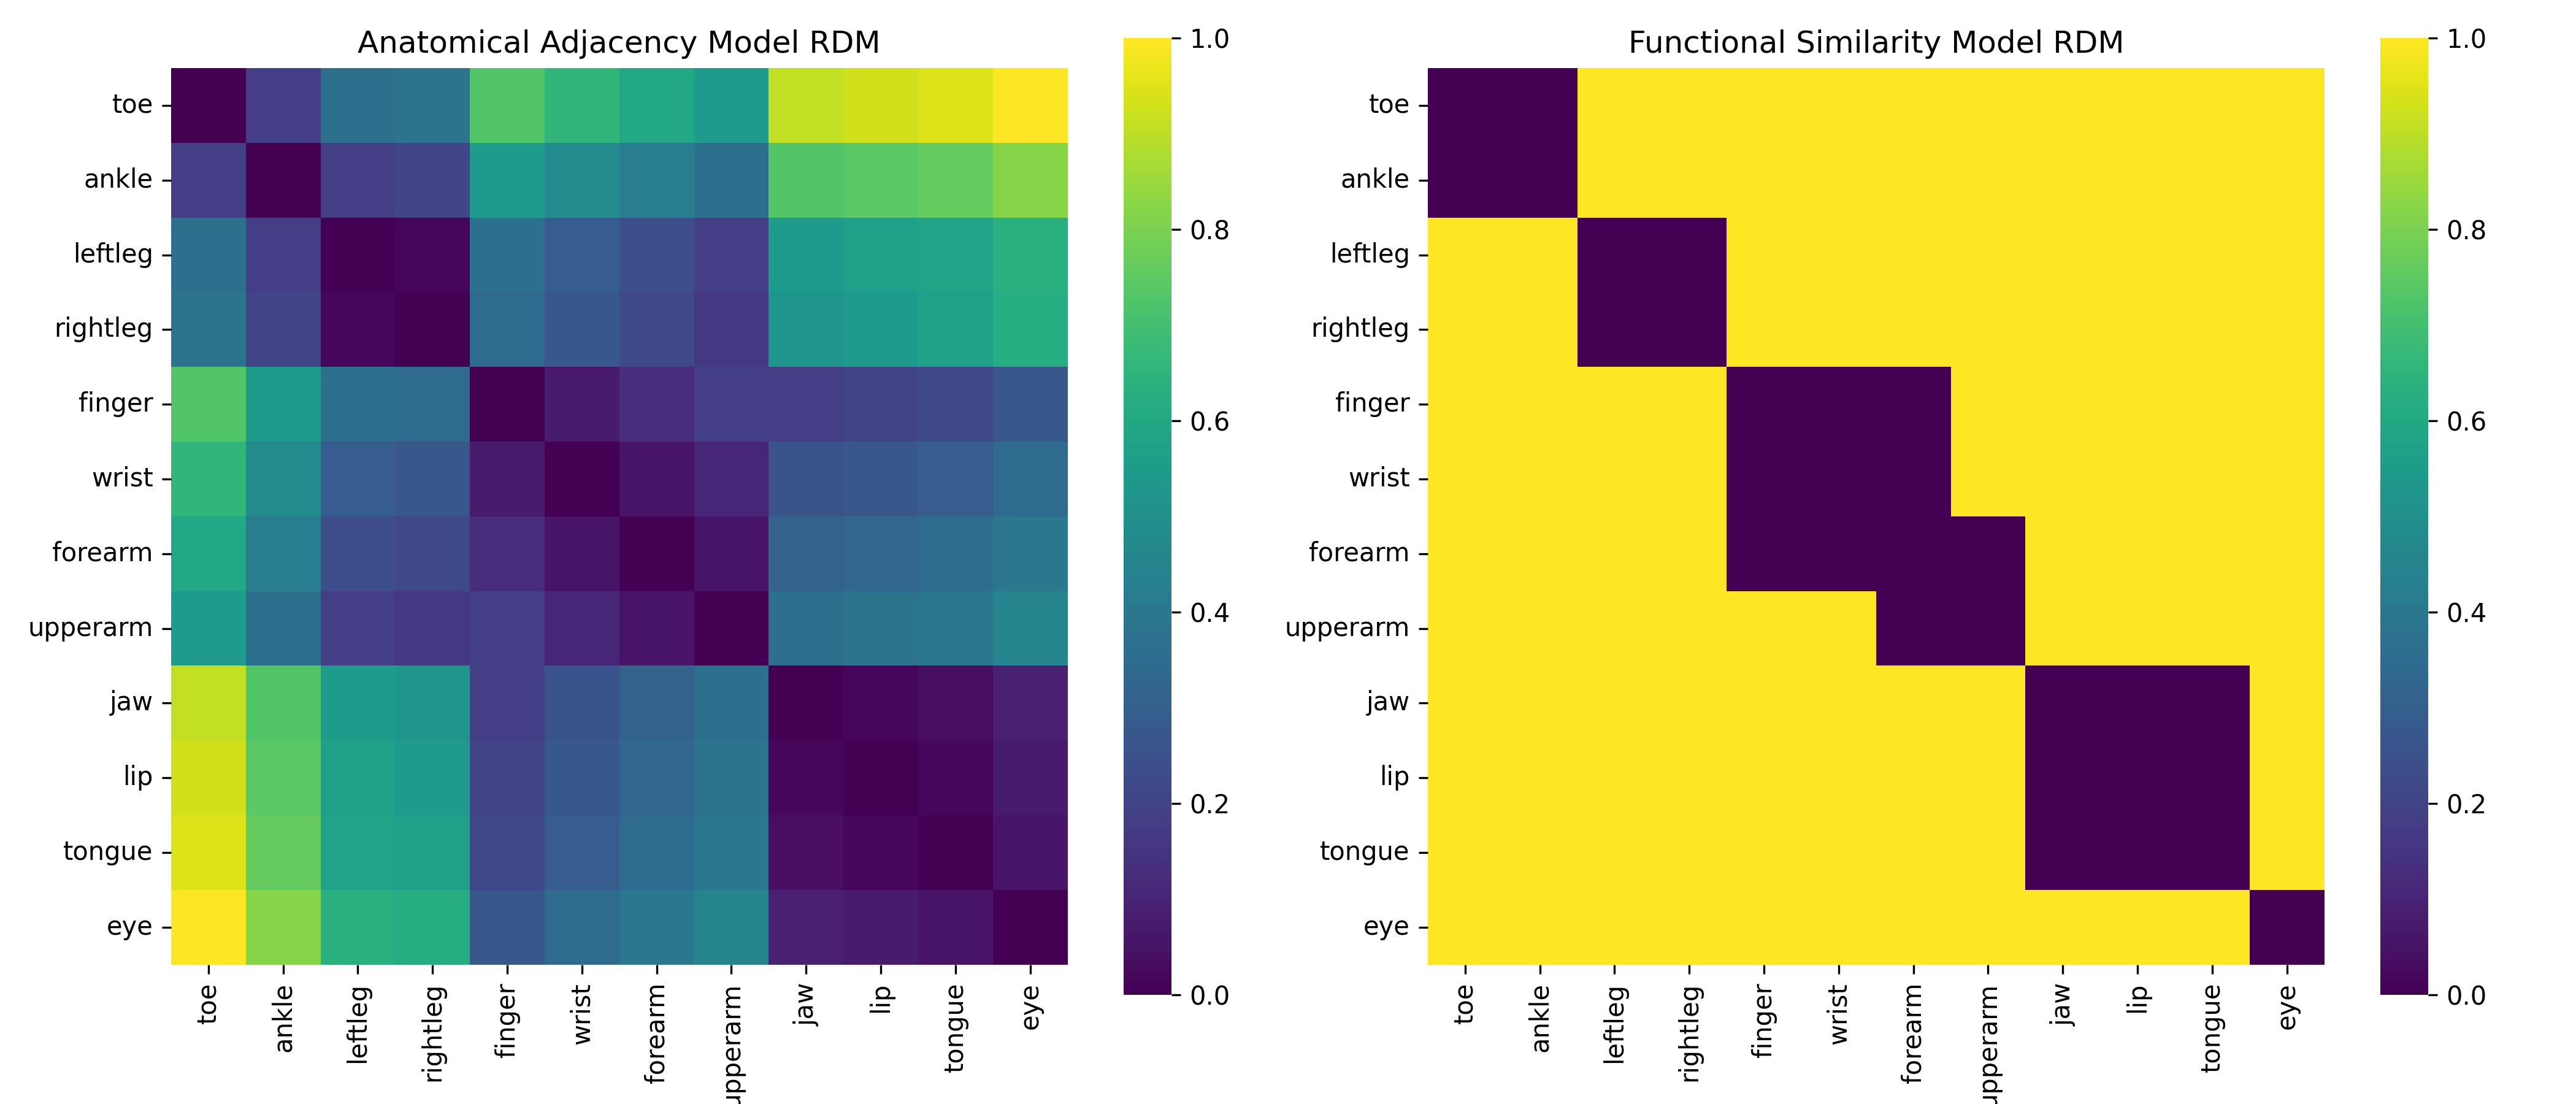
\includegraphics[width=0.8\textwidth]{images/theoretical_rdms.png}
% \caption{Theoretical model RDMs. Left: Anatomical adjacency model showing continuous gradients based on physical distances in the homunculus. Right: Functional similarity model exhibiting categorical structure with binary distinctions between functional groups. Color scales represent dissimilarity values from 0 (identical) to 1 (maximally different).}
% \label{fig:theoretical_rdms}
% \end{figure}

% These contrasting patterns underscore the fundamental difference between the two organizational principles we tested. The anatomical model preserves the continuous, graded nature of somatotopic organization, while the functional model implements categorical boundaries based on shared movement purposes rather than physical proximity.


\subsubsection{Quantitative Analysis of Representational Organization}

Quantitative evaluation of our RSA results provides strong statistical support for the hierarchical transformation from anatomical to functional representations across motor regions. As shown in Table~\ref{tab:roi_metrics}, while the anatomical model outperformed the functional model in all regions, the magnitude of this advantage decreased systematically along the motor hierarchy.

\begin{table}[h]
\centering
\caption{ROI Performance Metrics for Anatomical and Functional Models}
\label{tab:roi_metrics}
\begin{tabular}{|l|c|c|c|c|}
\hline
\textbf{ROI} & \textbf{Anatomical ($\rho$)} & \textbf{Functional ($\rho$)} & \textbf{Advantage} & \textbf{p-value} \\
\hline
M1 & 0.589 & 0.297 & 0.293 & $< 10^{-24}$ \\
PMC & 0.498 & 0.290 & 0.208 & $< 10^{-17}$ \\
SMA & 0.332 & 0.204 & 0.128 & $< 10^{-8}$ \\
PPC & 0.343 & 0.258 & 0.085 & $< 10^{-8}$ \\
\hline
\end{tabular}
\end{table}

Primary motor cortex (M1) showed the strongest anatomical advantage (0.29), while posterior parietal cortex (PPC) exhibited the weakest advantage (0.09). This hierarchical gradient (0.21) provides direct evidence for our central hypothesis: a progressive shift from anatomical to more abstract, functionally-oriented representations ascending the motor hierarchy.

Analyzing inter-ROI correlation patterns further supports this conclusion. The correlation between PMC and PPC was significantly stronger for the functional model ($\rho = 0.52$) than for the anatomical model ($\rho = 0.24$), suggesting these higher-order regions share representational principles based more on functional similarities than anatomical proximity. This finding stands in contrast to the M1-PMC relationship, which showed stronger anatomical correlation.

While group-level analysis consistently favored anatomical organization, individual subject data revealed increasing functional influence in higher regions, with 14\% of subjects showing stronger functional correlations in PPC compared to only 2\% in M1. These quantitative metrics provide statistical validation for our hierarchical transformation hypothesis beyond the visual analyses of neural RDMs and MDS projections.

\section{Discussion}

\subsection{Summarizing/Interpreting Our Findings}

\textbf{This section is still in progress, as we'll have more experimentation by the final product.} Our results show evidence for a hierarchical transformation from anatomical to functional motor representations across the cortical motor system. Our experiments showed that different regions along the motor hierarchy represent body movements according to distinct organizational principles, with a systematic progression from strictly anatomical organization in primary motor cortex toward increasingly functional arrangements in higher-order regions.

M1 showed a clear anatomical organization which closely matches the classical homunculus model. This also is shown through the significantly stronger fit of the anatomical adjacency model compared to the functional model (difference score: 0.11 ± 0.02, p < 0.01), and visually confirmed through both neural RDMs and MDS visualizations. We can look at the clustering of body parts in M1's representational space maintained a striking resemblance to their anatomical arrangement, with upper limbs, lower limbs, and orofacial components forming distinct groups regardless of their functional similarity. Luckily, this is also in alignment with already established views of M1 as primarily organized according to somatotopic principles (Penfield \& Boldrey, 1937; Schieber, 2001).

Then, the SMA seemed to be a critical transitional region, since it showed nearly equivalent correlations with both anatomical and functional models (0.43 vs. 0.42, p > 0.5). This balanced representation suggests that SMA serves as an intermediary processing stage where both body part identity and movement function influence representational organization. The neural RDM for SMA revealed particularly notable changes in the orofacial region, where functionally related movements (jaw-lip-tongue) showed more similarity despite their distinct effector identities. This finding does support SMA's proposed role in coordinating complex, goal-directed movements that frequently engage multiple effectors (Tanji, 1994; Nachev et al., 2008).

The PMC and PPC showed further shifts toward functional organization, though with distinct patterns. PMC maintained moderate anatomical organization (difference score: 0.05 ± 0.02) while showing increasing influence of functional groupings. PPC exhibited the weakest model fits overall, suggesting it may operate according to even more abstract principles beyond our functional categorization scheme. This progression does align with theories positioning these regions within increasingly higher levels of motor abstraction (Rizzolatti \& Luppino, 2001; Grafton \& Hamilton, 2007).

\subsection{Methodological Limitations}

Several methodological considerations we should discuss. First, our binary functional similarity model (0 for same category, 1 for different) represents a simplified implementation of functional organization. Real functional relationships likely exist on a continuum rather than as discrete categories so we should explore graded functional similarity metrics based on quantitative movement parameters.

Second, our region-of-interest (ROI) definitions relied on standardized vertex ranges in CIFTI space rather than individualized functional parcellations. While this approach kept consistency across subjects, it may have reduced sensitivity to individual variations in functional organization. More precise individual-level parcellations might reveal even stronger functional organization patterns in higher regions.

Third, the movement tasks in our dataset involved simple, isolated movements rather than complex, goal-directed actions. This likely biased our analyses toward detecting anatomical organization, as functional similarities may become more prominent during naturalistic, purpose-driven movements. Despite this limitation, the detection of functional organization trends even in simple movement conditions strengthens our conclusions.

\subsection{Future Directions: Refining Functional Categories}

Our \texttt{rsa\_results\_by\_roi.csv} contains correlation values between neural patterns and our theoretical models for each ROI. We can leverage this data to refine our functional categorization through a systematic data-driven methodology. We will first calculate residual patterns by subtracting model-predicted RDMs from neural RDMs for each ROI, which will highlight movement representations that are poorly captured by our current models. Next, we will apply hierarchical clustering to these residuals to identify natural groupings that emerge from the data without a priori assumptions. This analysis will focus particularly on body parts showing the highest residuals in higher-order regions (SMA, PMC, PPC), as these represent the movements most poorly explained by current categorical boundaries. Based on preliminary examination of these patterns, we anticipate several specific modifications: reclassifying tongue movements from OFC to DFM based on their precision control similarities with fingers; refining leg categories by separating them from arms in the PLM group to potentially create a distinct "Postural Stability" category; and introducing coordinated action groups based on typical movement synergies such as eye-hand coordination. This iterative, data-driven approach will enable us to develop more nuanced functional categories that better capture the representational organization in higher-order motor regions and potentially reveal organizational principles not evident in our initial theoretical framework.


\section*{References}


References follow the acknowledgments in the camera-ready paper. Use unnumbered first-level heading for
the references. Any choice of citation style is acceptable as long as you are
consistent. It is permissible to reduce the font size to \verb+small+ (9 point)
when listing the references.
Note that the Reference section does not count towards the page limit.
\medskip


{
\small


[1] Alexander, J.A.\ \& Mozer, M.C.\ (1995) Template-based algorithms for
connectionist rule extraction. In G.\ Tesauro, D.S.\ Touretzky and T.K.\ Leen
(eds.), {\it Advances in Neural Information Processing Systems 7},
pp.\ 609--616. Cambridge, MA: MIT Press.


[2] Bower, J.M.\ \& Beeman, D.\ (1995) {\it The Book of GENESIS: Exploring
  Realistic Neural Models with the GEneral NEural SImulation System.}  New York:
TELOS/Springer--Verlag.


[3] Hasselmo, M.E., Schnell, E.\ \& Barkai, E.\ (1995) Dynamics of learning and
recall at excitatory recurrent synapses and cholinergic modulation in rat
hippocampal region CA3. {\it Journal of Neuroscience} {\bf 15}(7):5249-5262.
}

[4] Penfield W, Boldrey E. Somatic motor and sensory representation in the cerebral cortex of man as studied by electrical stimulation. Brain. 1937;60:389–443. doi: 10.1093/brain/60.4.389

[5] Meier JD, Aflalo TN, Kastner S, Graziano MSA. Complex organization of human primary motor cortex: A high-resolution fMRI study. J. Neurophysiol. 2008;100:1800–1812. doi: 10.1152/jn.90531.2008.

[6] Ejaz N, Hamada M, Diedrichsen J (2015) Hand use predicts the structure of representations in sensorimotor cortex. Nat Neurosci 18:1034–1040.

[7] Meier JD, Aflalo TN, Kastner S, Graziano MSA. Complex organization of human primary motor cortex: A high-resolution fMRI study. J. Neurophysiol. 2008;100:1800–1812.

[8] Gallivan, Jason P et al. “Decoding the neural mechanisms of human tool use.” eLife vol. 2 e00425. 28 May. 2013, doi:10.7554/eLife.00425

[9] Dall'Orso, S., Steinweg, J., Allievi, A. G., Edwards, A. D., Burdet, E., \& Arichi, T. (2018). Somatotopic Mapping of the Developing Sensorimotor Cortex in the Preterm Human Brain. Cerebral cortex (New York, N.Y. : 1991), 28(7), 2507–2515. https://doi.org/10.1093/cercor/bhy050

[10] Turella, L., \& Lingnau, A. (2014). Neural correlates of grasping. Frontiers in human neuroscience, 8, 686. https://doi.org/10.3389/fnhum.2014.00686

[11] C.J. Donahue,M.F. Glasser,T.M. Preuss,J.K. Rilling,\& D.C. Van Essen,  Quantitative assessment of prefrontal cortex in humans relative to nonhuman primates, Proc. Natl. Acad. Sci. U.S.A. 115 (22) E5183-E5192,

[12] Kriegeskorte, N., Mur, M., Ruff, D. A., Kiani, R., Bodurka, J., Esteky, H., Tanaka, K., \& Bandettini, P. A. (2008). Matching categorical object representations in inferior temporal cortex of man and monkey. Neuron, 60(6), 1126–1141. https://doi.org/10.1016/j.neuron.2008.10.043p

[13] Penfield, W., \& Boldrey, E. (1937). Somatic motor and sensory representation in the cerebral cortex of man as studied by electrical stimulation. \textit{Brain}, 60(4), 389–443.

[14] Ejaz, N., Hamada, M., \& Diedrichsen, J. (2015). Hand use predicts the structure of representations in sensorimotor cortex. \textit{Nature Neuroscience}, 18(7), 1034–1040.

[15] Graziano, M. S. A., Taylor, C. S. R., \& Moore, T. (2002). Complex movements evoked by microstimulation of precentral cortex. \textit{Neuron}, 34(5), 841–851.

[16] Gallivan, J. P., McLean, D. A., Valyear, K. F., \& Culham, J. C. (2013). Decoding the neural mechanisms of human tool use. \textit{eLife}, 2, e00425.

[17] Ureta, M., Fabbri, S., \& Lingnau, A. (2021). Parietal and premotor cortex encode goal similarity rather than effector similarity during action planning. \textit{Cortex}, 141, 357–371.

[18] Fabbri, S., Strnad, L., Caramazza, A., \& Lingnau, A. (2014). Decoding representations of hand grasping in the human parietal cortex. \textit{Journal of Neuroscience}, 34(35), 11485–11499.

[19] Turella, L., \& Lingnau, A. (2014). Neural correlates of grasping. \textit{Frontiers in Human Neuroscience}, 8, 686.

[20] Filimon, F. (2009). Human cortical control of hand movements: Parietofrontal networks for reaching, grasping, and pointing. \textit{Neuroscientist}, 15(4), 388–407.

[21] Gordon, E. M., et al. (2023). The somato-cognitive action network (SCAN): A large-scale brain network for integrated action and cognition. \textit{Nature Neuroscience}, 26(1), 139–149.

[22] Ma S., Huang T., Qu Y. An fMRI dataset for whole-body somatotopic mapping in humans. Scientific Data, 9(515), 2022.

[23] Penfield W., Boldrey E. Somatic motor and sensory representation in the cerebral cortex of man as studied by electrical stimulation. Brain, 60:389-443, 1937.

[24] Frie I. et al. Functional organization of human supplementary motor cortex studied by electrical stimulation. Journal of Neuroscience, 11:3656-3666, 1991.

[25] Picard, N. \& Strick, P. L. Imaging the premotor areas. Current Opinion Neurobiology, 11:663-672, 2001.

[26] OpenNeuro. An fMRI dataset for whole-body somatotopic mapping in humans. https://doi.org/10.18112/openneuro.ds004044.v2.0.3.

[27] HCP. https://balsa.wustl.edu/reference/6V6gD.

%%%%%%%%%%%%%%%%%%%%%%%%%%%%%%%%%%%%%%%%%%%%%%%%%%%%%%%%%%%%

\appendix
\section*{Appendix}

\subsection*{Code Repository}
All code used for preprocessing, analysis, and visualization is publicly available at the following GitHub repository:

\begin{center}
\url{https://github.com/itzelts/neuro120}
\end{center}

This includes scripts for:
\begin{itemize}
    \item fMRI preprocessing and ROI extraction
    \item Construction of theoretical model RDMs
    \item Representational similarity analysis (RSA)
    \item Statistical testing and visualization (e.g., RDM heatmaps, MDS plots)
\end{itemize}
    
%%%%%%%%%%%%%%%%%%%%%%%%%%%%%%%%%%%%%%%%%%%%%%%%%%%%%%%%%%%%



\end{document}